\chapter{Introduction} \label{chap:intro}
A gentle reminder not to get this chapter perfect until the dissertation is nearing its completion\ldots

\section{A section}

\subsection{A sub-section}

\subsubsection{A sub-sub-section}



\section{Citations}

When it comes to referencing, if we want to assert a fact and then provide its reference use \verb!\parencite!. For example -- one should adapt feedback to learner personality \parencite{dennis2016adapting}.

Or if you want to talk about the research directly, use \verb!\textcite!: \textcite{dennis2016adapting} did a PhD in adapting feedback to learner personality. 

If you want to cite two sources at the same time, you can separate the keys with commas \parencite{dennis2016adapting,cle12}.

\section{Figures}

\begin{figure}
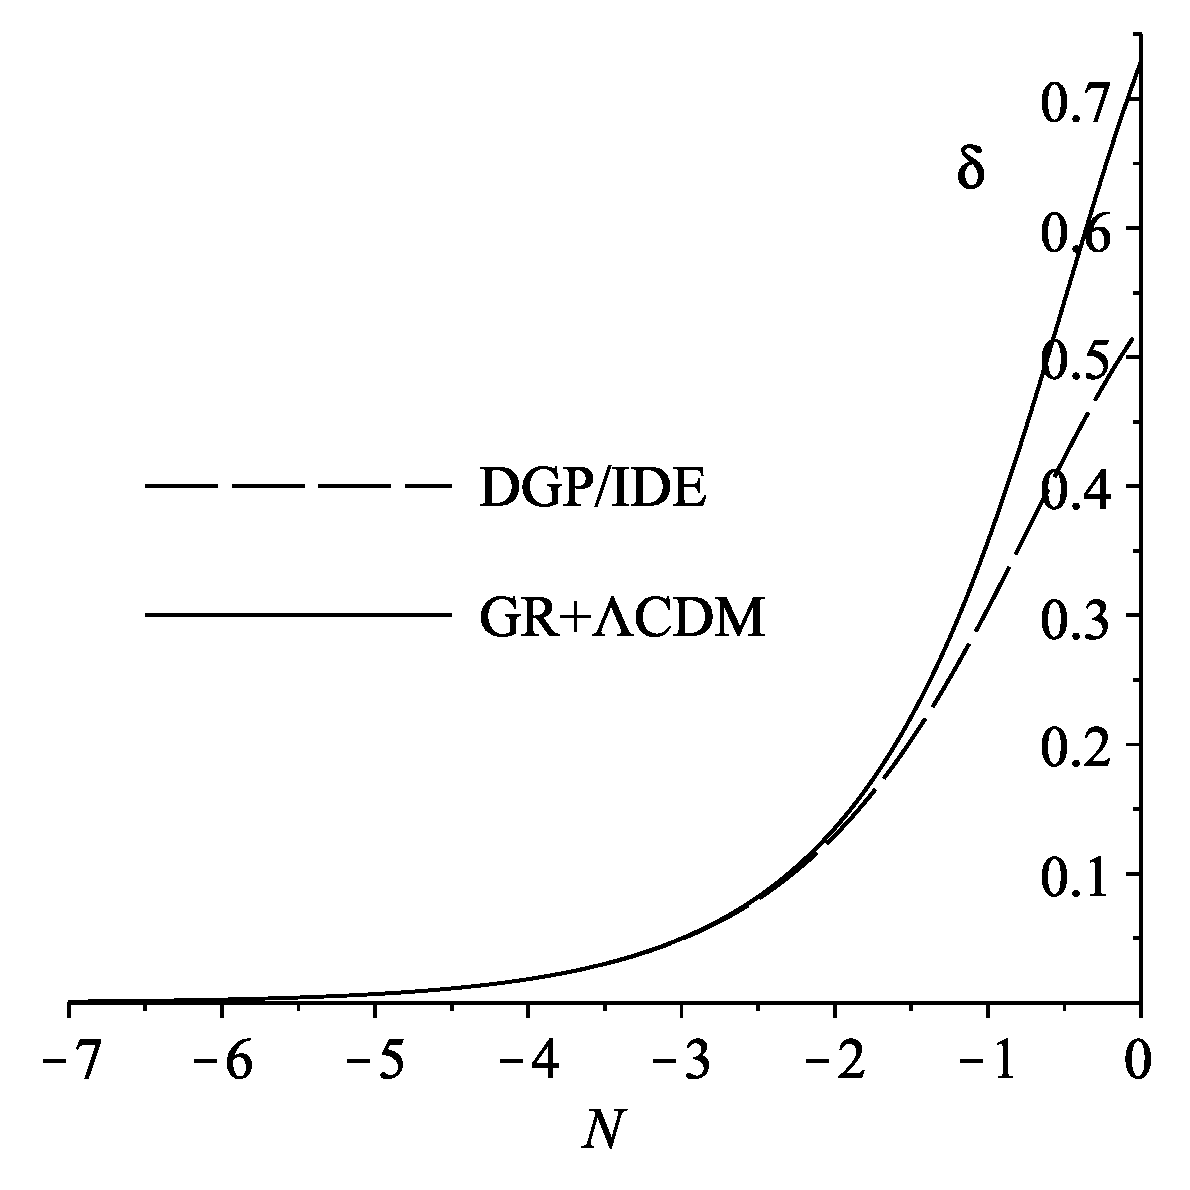
\includegraphics[width=0.49\columnwidth]{figures/dgpdeltas.eps}
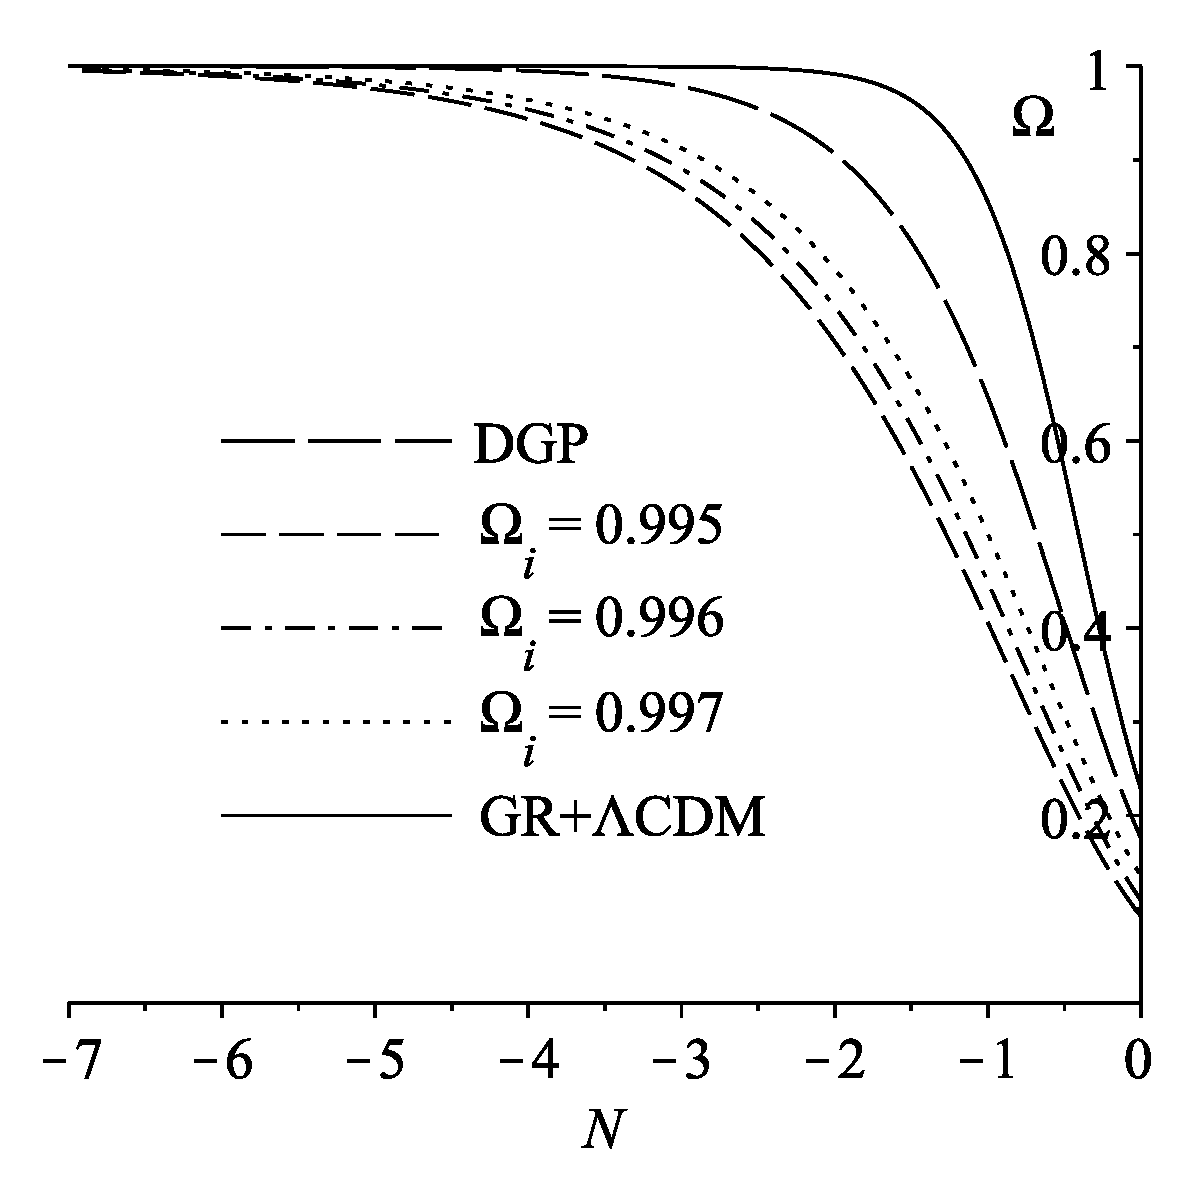
\includegraphics[width=0.49\columnwidth]{figures/dgpomegas.eps}
% For long captions include a short version for the List of Figures/Tables sections in square brackets as below.
\caption[Evolutions of $\delta$ and $\Omega$ for DGP]{Evolution of the density perturbation (left) and the density parameters (right) for the matched DGP/IDE models, each with a different $\Omega_i$,
and a GR+$\Lambda$CDM model.
\label{fig:matched}}
\end{figure}

Don't the graphs in \autoref{fig:matched} look scary? Don't worry, this is because I adapted this template from ICJS. Remember - if you are including screenshots or other raster graphics (i.e. PNG, JPEG) you should ensure that they are at least 300dpi. This will take effort on your part - most people's screens are at 72dpi.   

Vector is better (EPS or PDF) if you can manage it. If you are exporting graphs from Microsoft Excel for example, place the chart in its own sheet and print it to PDF. Then, using Acrobat or similar, crop the whitespace off the PDF. This is the most reliable way I have found to include vector graphics from Microsoft Office.







% To include math symbols in things with hyperlinks you need to specify an alternative plain text version for the bookmark using \texorpdfstring as below:
\section{A section with math symbols, eg. \texorpdfstring{$\Lambda$}{Lambda}CDM}
test test test test test test test test test test test test test test test test test test test test test test test test test test test test test test test test test test test test test test test test
test test test test test test test test test test test test test test test test test test test test test test test test test test test test test test test test test test test test test test test test
test test test test test test test test test test test test test test test test test test test test test test test test test test test test test test test test test test test test test test test test
test test test test test test test test test test test test test test test test test test test test test test test test test test test test test test test test test test test test test test test test

